\documentclass[11pt,a4paper]{jsarticle}
% template at 「TeXテンプレート - [物理のかぎしっぽ]」 http://hooktail.org/computer/index.php?TeX%A5%C6%A5%F3%A5%D7%A5%EC%A1%BC%A5%C8
%
\usepackage{amsmath,amssymb}
\usepackage{graphicx}
%
\setlength{\textwidth}{\fullwidth}
\setlength{\textheight}{40\baselineskip}
\addtolength{\textheight}{\topskip}
\setlength{\voffset}{-0.2in}
\setlength{\topmargin}{0pt}
\setlength{\headheight}{0pt}
\setlength{\headsep}{0pt}

\newcommand{\argmin}{\mathop{\rm argmin}\limits}
\newcommand{\argmax}{\mathop{\rm argmax}\limits}
\newcommand{\V}[1]{\boldsymbol{#1}}
%
%
\title{graph-based SLAMの解説}
\author{上田 隆一}
\date{\today}
\begin{document}

\maketitle

\footnote[0]{\copyright\ 2017 Ryuichi Ueda}
%
%
\section{はじめに}

この文章は、\cite{grisetti2010}などのチュートリアルを見ても数式の細かいところが分からない
graph-based SLAMについて、
実際の計算方法を細かく解説するためのものである。
実装例はGitHubの\texttt{ryuichiueda/probrobo\_practice}
の\texttt{./graph-based\_SLAM/graph-based\_slam.ipynb}にあり、
この文章はこの実装の数学的な解説となる。
ただし、コードで使った記号と本文章の記号は一部異なる。

\section{問題}

%対向二輪型(その場で回転できるロボット)で、
平面上を移動し、向きを持ち、カメラでランドマーク観測ができるロボットで
graph-based SLAMを実行する方法を考える。ランドマークは環境にいくつか存在し、
ロボットからは互いに識別でき、距離と見える方角が観測できる。
また、2つの観測がどの方角から観測されたものか、相対的に分かるものとする。

\subsection{ロボットの姿勢と座標系}\label{sub:pose}

世界座標系$\Sigma_\text{w}$におけるロボットの姿勢(位置と向き)を
\begin{align}
	\V{x} =
	\begin{bmatrix}
		x \\ y \\ \theta
	\end{bmatrix}
\end{align}
で表す。また、$[x\ y]^T$を原点として、$X$軸が世界座標系で$\theta$の方向を向いているロボット座標系
$\Sigma_\text{r}$を考える。これらの関係を図\ref{fig:coordinate}に示す。

\begin{figure}[htbp]
	\begin{center}
		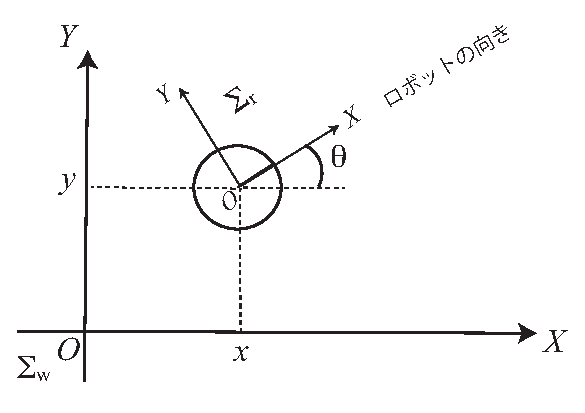
\includegraphics[width=0.5\linewidth]{./figs/coordinate.eps}
		\caption{世界座標系とロボットの姿勢}
		\label{fig:coordinate}
	\end{center}
\end{figure}

%\subsection{ロボットの運動}

離散的な時刻$t = 0,1,2,\dots,T$を考える。
時刻の集合を$\mathcal{T}$で表す。
時刻$t$における世界座標系でのロボットの姿勢の真値を$\V{x}_t^*$で表す。
ロボットはデッドレコニングで$\V{x}_t$の推定値$\hat{\V{x}}_t$を認識するが、
ロボットの動作は雑音の影響を受けるため、
$\V{x}_t^*$と$\hat{\V{x}}_t$の間には誤差が発生する。


ロボットは一つの行動ごとに$\hat{\V{x}}_t$を記録していく。
全時刻の推定姿勢を
\begin{align}
\hat{\V{x}}_{0:T} = \{\hat{\V{x}}_0, \hat{\V{x}}_1, \dots, \hat{\V{x}}_T \}
\end{align}
と表すこととする。

\subsection{観測}

環境中にいくつかランドマークが存在していると仮定する。
時刻$t$におけるロボット座標系$\Sigma_\text{r}$を$\Sigma_{\text{r}t}$と表すこととすると、
ロボットには、時刻$t$において、全ランドマークのうちいくつかを計測する。

\subsubsection{ランドマークの識別}

ロボットからは、一度観測したランドマークは、後の時刻で観測したときに、どのランドマークか
識別できることとする。ロボットは観測したランドマークにIDを与えて管理することにする。
IDは$c$と表し(番号でも文字列でもなんでも良い)、IDとして$c$を与えられたランドマークを
$L_c$と表す。
ロボットが認識しているランドマークのIDの集合を$C$で表す。

\subsubsection{ランドマークの姿勢計測}

ロボットは$\Sigma_{\text{r}t}$においてランドマーク$L_c$を観測したとき、
$L_c$までの距離$d_{c,t}$と、ランドマークが見える方向$\varphi_{c,t}$を計測値として得る。
また、ランドマークも方角を持ち(ロボットの$\theta$に相当)、
ロボットに対してどの方角を向いているか分かることとする。
この値を$\psi_{c,t}$とする\footnote{この仮定は実用上強すぎるが、
実際には、後の計算式から分かるように、
2つの姿勢間での値$\psi_{c,t}, \psi_{c,t'}$の差だけが分かれば良い。
例えば、2点間で得られた画像の向きを画像処理から割り出すなどの処理で、この差は得られる。}。
図\ref{fig:observation}にこれらの記号の関係を示す。

\begin{figure}[htbp]
	\begin{center}
		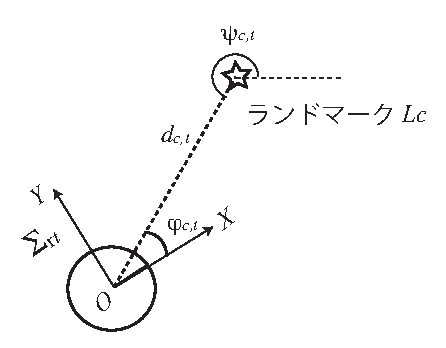
\includegraphics[width=0.5\linewidth]{./figs/observation.eps}
		\caption{計測値}
		\label{fig:observation}
	\end{center}
\end{figure}

\subsubsection{計測値の記録}

ロボットが時刻$t$で得るランドマーク全ての計測値の集合は、
$Z_t = \{ \V{z}_{c,t} = (d_{c,t}, \varphi_{c,t}, \psi_{c,t}) |
c \in C, c\text{: 観測したランドマークのID} \}$
で表すことができ、これもロボットは各時刻ごとに記録する。
$Z_t$の集合を$Z_{0:T}$で表す。

\subsubsection{計測値の誤差}\label{sub:noise}

ランドマーク観測から得られる計測値には正規分布に従う雑音が混入すると仮定する。
また、ロボットは雑音の傾向を知っていることとする。

$d_{c,t}$には、10[\%]の雑音が混入する\footnote{$「10$[\%]」は変数にすべきだが、
記号が増えて理解の妨げになるので固定値として説明する。}。
正確には真値を$d_{c,t}^*$とすると、
\begin{align}
	d_{c,t} \sim \mathcal{N}\left(d_{c,t}^*,(d_{c,t}^*/10)^2\right) \label{eq:ddist}
\end{align}
にしたがって$d_{c,t}$が生成される。ここで$\mathcal{N}(\mu,\sigma^2)$は
平均値$\mu$、標準偏差$\sigma$の正規分布を表す。

また、$\varphi_{c,t},\psi_{c,t}$にも$3\pi/180$[rad]の標準偏差で雑音が混入する。
これらの真値をそれぞれ$\varphi_{c,t}^*,\psi_{c,t}^*$とすると、
$\varphi_{c,t},\psi_{c,t}$は、
\begin{align}
	\varphi_{c,t} \sim \mathcal{N}\left(\varphi_{c,t}^*,(3\pi/180)^2\right) \label{eq:phidist}\\
	\psi_{c,t} \sim \mathcal{N}\left(\psi_{c,t}^*,(3\pi/180)^2\right) \label{eq:psidist}
\end{align}
で生成される。


\subsection{ポーズ調整}\label{sub:fullslam}

ここで、$Z_{0:T}$、デッドレコニングでの計測値$\hat{\V{x}}_{0:T}$から、
真値$\V{x}_{0:T}^*$を推定する問題を考える。
この問題を、
任意のロボットの軌跡$\V{x}_{0:T}$がどれだけ$Z_{0:T}$を説明するかを
評価関数として定式化し、この評価関数を用いた最適化問題として定義する。
この評価関数については、次章の実装の中で説明する。


\section{graph-based SLAMの実装例}

実装の一例を示す。

\subsection{グラフのエッジを作る}

問題を解くために、次のノード(頂点)、
エッジ(辺、アーク)を持つグラフを考える。
ノードはロボットの各時刻の姿勢に対応し、
エッジは、同じランドマークを計測した2つのノード間に設けられる。

各ノードは、ロボットの各時刻の推定姿勢$\V{x}_{0:T}$を変数として有する。
これらの推定姿勢は計算の途中で変化していくが、
その初期値はデッドレコニングから得られた$\hat{\V{x}}_{0:T}$
とする。

エッジは、両端の2つのノードについて、
2つのランドマーク観測から計算できる2つのノードの
相対姿勢を表すベクトル$\V{\mu}_{c,t,t'}$
その正確さを情報として持つ。
ベクトル$\V{\mu}_{c,t,t'}$は、
時刻$t$の姿勢から時刻$t'$の姿勢への向きを正とする。
また、「正確さ」というのは世界座標系での情報行列$\Omega_{c,t,t'}$
で表現される。情報行列とは共分散行列の逆行列で、
$\Omega_{c,t,t'}$を計算する際の共分散行列$\Sigma_{c,t,t'}$は、
\ref{sub:noise}項でモデル化した雑音から計算する。
計算方法は後述する。

このようなグラフを作ると、1つのエッジと両端のノードは、
\begin{itemize}
	\item エッジの持つ$\mu_{c,t,t'}$
	\item 両ノードの持つ推定姿勢の差$\V{x}_{t'} - \V{x}_t$
\end{itemize}
の、2つの重複した相対姿勢の情報を持つことになる。
この1つのエッジと両端のノードに話を限ると、
推定姿勢$\V{x}_{t'},\V{x}_t$を変化させて、
次の誤差
\begin{align}
	\V{e}_{c,t,t'} = \V{x}_t' - \V{x}_t - \V{\mu}_{c,t,t'}\label{eq:e}
\end{align}
をゼロにすると、推定姿勢がランドマーク観測の計測値を最も
説明するものになる。
一方、ノードは他のエッジとも繋がっているので、
こちらだけをゼロに合わせると別のエッジでの誤差が増えるため、
全体として最適な推定姿勢を探さなければならない。



%共分散行列の逆行列は一般に情報行列と呼ばれる。$\Omega_{c,t,t'}$は、
%ランドマーク観測から2地点の変位を計算したときの信頼性を表す。


\subsubsection{$\V{\mu}_{c,t,t'}, \V{e}_{c,t,t'}$の計算}

2つの時刻$t,t'$で同じランドマーク$L_c$を観測したときのロボットとランドマークの
幾何的な関係を図\ref{fig:two_poses}に示す。
二つの観測を図の点線の矢印のように世界座標系にベクトルとして描くと、
時刻$t$の観測のベクトルに、時刻$t'$の観測のベクトルの
向きを反転して足せば$\V{\mu}_{c,t,t'}$が求まることが分かる。


\begin{figure}[htbp]
	\begin{center}
		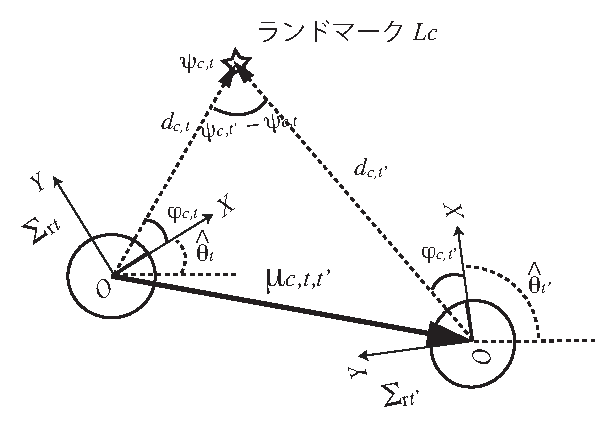
\includegraphics[width=0.5\linewidth]{./figs/two_poses.eps}
		\caption{ランドマークの計測値から2点の相対姿勢を求める}
		\label{fig:two_poses}
	\end{center}
\end{figure}

したがって、$\V{\mu}_{c,t,t'}$($x,y,\theta$座標のベクトルとなる)
は次のような単純な幾何計算で求まる
\footnote{おそらく$\psi$は$\theta$で置き換えられるので
$\psi$を使わない実装もできるが、まだ自分自身では検証していない。}。
\begin{align}
	\V{\mu}_{c,t,t'} =
	\begin{bmatrix}
	d_{c,t} \cos(\theta_t + \varphi_{c,t}) \\
	d_{c,t} \sin(\theta_t + \varphi_{c,t}) \\
	\psi_{c,t}
	\end{bmatrix}
	- 
	\begin{bmatrix}
	d_{c,t'} \cos(\theta_{t'} + \varphi_{c,t'}) \\
	d_{c,t'} \sin(\theta_{t'} + \varphi_{c,t'}) \\
	\psi_{c,t'}
	\end{bmatrix}
\end{align}

また、式(\ref{eq:e})から、
\begin{align}
	\V{e}_{c,t,t'} &= \V{x}_{t'} - \V{x}_t -
	\begin{bmatrix}
	d_{c,t} \cos(\theta_t + \varphi_{c,t}) \\
	d_{c,t} \sin(\theta_t + \varphi_{c,t}) \\
	\psi_{c,t}
	\end{bmatrix} 
	+ 
	\begin{bmatrix}
	d_{c,t'} \cos(\theta_{t'} + \varphi_{c,t'}) \\
	d_{c,t'} \sin(\theta_{t'} + \varphi_{c,t'}) \\
	\psi_{c,t'}
	\end{bmatrix} \nonumber \\
	&= 
	\begin{bmatrix}
		x_{t'} - x_t 
		- d_{c,t} \cos(\theta_{t} + \varphi_{c,t}) + d_{c,t'} \cos(\theta_{t'} + \varphi_{c,t'}) \\
		y_{t'} - y_t 
		- d_{c,t} \sin(\theta_{t} + \varphi_{c,t}) + d_{c,t'} \sin(\theta_{t'} + \varphi_{c,t'}) \\
		\theta_{t'} - \theta_t 
	- \psi_{c,t} + \psi_{c,t'}
	\end{bmatrix} \label{eq:e2}
\end{align}
となる。

\subsubsection{$\Sigma_{c,t,t'}, \Omega_{c,t,t'}$の計算}

共分散行列$\Sigma_{c,t,t'}$は、$t$、$t'$におけるランドマーク$L_c$
の計測の誤差に関する共分散行列$\Sigma_{c,t}, \Sigma_{c,t'}$
をそれぞれの計測座標系で求め、世界座標系に座標変換(回転)して足し合わせたものとなる。
ここで言う「計測座標系」とは、ロボットからランドマークが計測された向きに引いた線を
$X$軸とする座標系である。図\ref{fig:observation_noise}に、
ロボット座標系、計測座標系の関係と、ランドマークの計測値の誤差に関する共分散行列を示す。

\begin{figure}[htbp]
	\begin{center}
		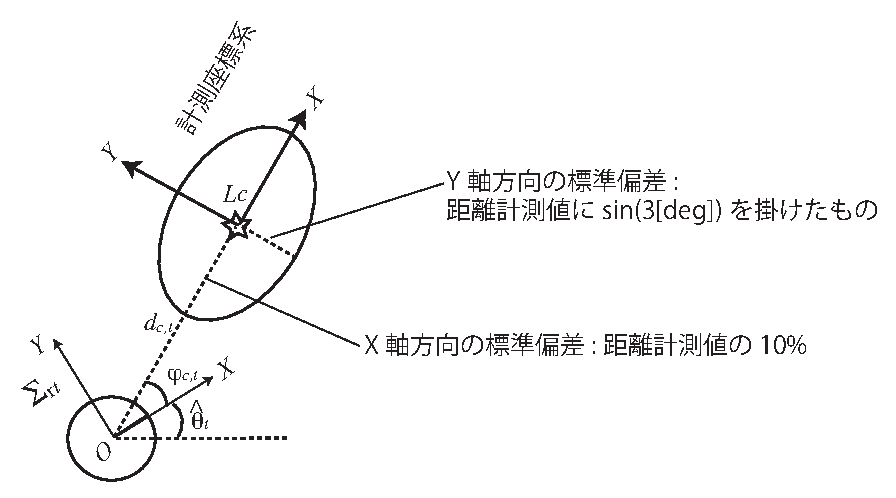
\includegraphics[width=0.8\linewidth]{./figs/observation_noise.eps}
		\caption{ランドマークの計測値の不確かさを表す共分散行列}
		\label{fig:observation_noise}
	\end{center}
\end{figure}


時刻$t$での$L_c$の計測に関する雑音を計測値周りのガウス分布で表すと、
計測座標系におけるこの分布の共分散行列$\Sigma_{c,t}$は、次のようになる。
\begin{align}
	\Sigma_{c,t} =
	\begin{bmatrix}
	(d_{c,t}/10)^2 & 0 & 0 \\
	0 & [(d_{c,t}/10)\sin(3\pi/180)]^2 & 0 \\
	0 & 0 & (3\pi/180)^2\cdot 2
	\end{bmatrix}
\end{align}
対角成分はそれぞれ計測座標系での$X,Y$軸、
$\theta$方向の共分散であり、式(\ref{eq:ddist}-\ref{eq:psidist})
の分布の分散に由来する。$Y$軸の共分散は、ランドマークの向きの計測誤差に、
距離の計測値を掛けたものになる
\footnote{小さい角度なので、$\sin(3\pi/180)$は$3\pi/180$に近似しても良い。}。
また、$\theta$方向の共分散については、$\phi,\psi$の計測の雑音両方が
不確かさの原因になるので、分散の値は一方のものの倍になる。

次に、計測座標系で計算した$\Sigma_{c,t}$を世界座標系の誤差楕円に変換する。
デッドレコニングの値、ランドマークの計測値から、
計測座標系は世界座標系から$\theta_{t'} + \varphi_{c,t'}$だけ
回転しているとみなすことができるので、$\Sigma_{c,t}$をこの角度だけ回転してやればよい。
この回転行列は、
\begin{align}
	R_{c,t} &=
	\begin{bmatrix}
	c & s  & 0 \\
	-s & c & 0 \\
	0 & 0 & 1
	\end{bmatrix}
\end{align}
となる。ここで、
\begin{align}
	c &= \cos(\theta_{t} + \varphi_{c,t}) \nonumber \\
	s &= \sin(\theta_{t} + \varphi_{c,t}) \nonumber 
\end{align}
である。この回転行列を$\Sigma_{c,t}, \Sigma_{c,t'}$に対してそれぞれ求めると、
\begin{align}
	\Sigma_{c,t,t'} &= R_{c,t}\Sigma_{c,t}R_{c,t}^T + R_{c,t'}\Sigma_{c,t'}R_{c,t'}^T \\
	\Omega_{c,t,t'} &= \Sigma_{c,t,t'}^{-1}
\end{align}
となる。この時点で$\Sigma_{c,t,t'}$の各要素は、
全て既知の値から計算された実数になっているはずである。

\subsection{最適化問題を作る}

\ref{sub:fullslam}節で棚上げした問題定義を行う。
まず、ロボットがオンラインで得たデータから得られる全通りの
$\V{e}_{c,t,t'}$で集合$\mathcal{E}$を作る。
このとき、$\mathcal{E}$の中の各要素がゼロベクトルになるように
$\V{x}_{0:T}$を$\V{\mu}_{c,t,t'}$に近づけていくと、
ランドマーク観測で得られた計測値を説明するロボットの軌跡
$\V{x}_{0:T}$が得られる。
しかし、ランドマーク観測で得られた計測値には雑音が含まれ、
全ての計測値と一致するような軌跡は得られない。
また、\ref{sub:noise}項の定義では、遠いところでランドマークを
観測した時の距離の計測値$d$と、近いところで計測した時の$d$では、
近いところで計測したものの方が精度が良くなる。
そのため、遠いところの計測値と近いところの計測値が互いに矛盾しているときは、
軌跡の推定の際は近いところの計測値を優先するべきである。

\subsubsection{マハラノビス距離}

以上を勘案する上で、情報行列$\Omega_{c,t,t'}$、ベクトル$\V{e}_{c,t,t'}$に対して
次のような値を考えることは有用である。
\begin{align}
	f_{\Omega_{c,t,t'}}(\V{x}_t,\V{x}_{t'}) = \V{e}_{c,t,t'}^T \Omega_{c,t,t'} \V{e}_{c,t,t'}
\end{align}
この値はマハラノビス距離を二乗した値である。
マハラノビス距離は、誤差のベクトル$\V{e}$の二乗誤差を計算するときに、
ただ内積$\V{e}^T \V{e}$を計算するのではなく、
間に情報行列を入れて重みをつけたものと解釈できる。
%例えば、共分散行列の各要素の値が大きくなると、
%その逆行列である情報行列は小さくなるので、$f$の値は小さくなる。
1次元で考えると、同じ大きさの誤差に対し、
共分散が大きいと(つまり誤差が大きいと予想される場合)
マハラノビス距離が小さくなり、
共分散が小さいとマハラノビス距離が大きくなる。

\subsubsection{最適化する式}

各ベクトル$\V{e}_{c,t,t'}$に対して、
マハラノビス距離の二乗の和: 
\begin{align}
	F(\V{x}_{0:T}) = \sum_{\V{e}_{c,t,t'} \in \mathcal{E}} \V{e}_{c,t,t'}^T \Omega_{c,t,t'} \V{e}_{c,t,t'}
\end{align}
を最小にする最適化問題を考える。
このようにマハラノビス距離を用いることで、
ランドマークの計測値が信頼できる
(この場合では近いところでランドマークを観測したときの計測値で
構成される)エッジの影響が、信頼できないエッジよりも誤差に対して
$F$の変化に大きな影響を与えるため、
姿勢を推定するときに優先される。

\subsection{$\V{e}_{c,t,t'}$の勾配を求める}

$\V{x}_t$と$\V{x}_{t'}$を変化させたときに
$\V{e}_{c,t,t'}$がどれだけ変化するかを求める。
まず、$\V{x}_t$と$\V{x}_{t'}$を連結したベ6次元のベクトル
\begin{align}
	\V{x}_{tt'} &= [ \V{x}_t \ \V{x}_{t'} ]^T \nonumber \\
	&= [ x_t \ y_t \ \theta_t \ x_{t'} \ y_{t'} \ \theta_{t'} ]^T \nonumber
\end{align}
を考える。これを$\Delta\V{x}$だけ微小変化させたときの
$\V{e}_{c,t,t'}$($\V{x}_{tt'}$と同じ変数を持つ
6次元ベクトル$\V{x}$の関数とみなす)の変化量は、次の近似で説明できる。
\begin{align}
	\V{e}_{c,t,t'}(\V{x}_{tt'} + \Delta\V{x}) 
	= \V{e}_{c,t,t'}(\V{x}_{tt'}) 
	+ \dfrac{\partial \V{e}_{c,t,t'}}{\partial \V{x}} \Big|_{\V{x} = \V{x}_{tt'}} \Delta\V{x}
\end{align}
ここでヤコビ行列$\dfrac{\partial \V{e}_{c,t,t'}}{\partial \V{x}} \Big|_{\V{x} = \V{x}_{tt'}}$を
$J_{c,t,t'}$と表すと、
\begin{align}
	J_{c,t,t'} = 
	\begin{bmatrix}
		-1 &  0 & d_{c,t} \sin(\theta_t + \varphi_{c,t}) & 1 & 0 & -d_{c,t'} \sin(\theta_{t'} + \varphi_{c,t'})\\
		 0 & -1 & -d_{c,t} \cos(\theta_t + \varphi_{c,t}) & 0 & 1 & d_{c,t'} \cos(\theta_{t'} + \varphi_{c,t'})\\
		 0 &  0 & -1                                     & 0 & 0 & 1 
	\end{bmatrix}
\end{align}
となる。後の計算のため、この行列の左半分と右半分を分けて、
\begin{align}
	A_{c,t,t'} &= 
	\begin{bmatrix}
		-1 &  0 & d_{c,t} \sin(\theta_t + \varphi_{c,t}) \\
		 0 & -1 & -d_{c,t} \cos(\theta_t + \varphi_{c,t}) \\
		 0 &  0 & -1                                    
	\end{bmatrix} \\
	B_{c,t,t'} &= 
	\begin{bmatrix}
		 1 & 0 & -d_{c,t'} \sin(\theta_{t'} + \varphi_{c,t'})\\
		 0 & 1 & d_{c,t'} \cos(\theta_{t'} + \varphi_{c,t'})\\
		 0 & 0 & 1 
	\end{bmatrix}
\end{align}
を定義しておく。この二つの行列は、最適化問題を解く際に、
それぞれ$\V{x}_t, \V{x}_{t'}$をどの方向に動かすと
$f_{\Omega_{c,t,t'}}(\V{x}_t,\V{x}_{t'})$
の変化量が大きいかという情報を持っている。


\subsection{問題を解く}


まず、$3(T+1)$行$3(T+1)$列の大きな情報行列$H$を考える。
$H$の各要素は、$\V{x}_{0:T}$の各変数に対応する。
この情報行列には、各エッジの誤差の情報を足し込んでいく。
具体的には、$H$の時刻$i$に対応する3行と、時刻$j$に対応する3列で
構成される$3\times3$の部分行列$H_{[ij]}$を考えたとき、
次のように各エッジのデータを足し込んでいく。
\begin{align}
	H_{[tt]} &\longleftarrow H_{[tt]} + A_{c,t,t'}^T \Omega_{c,t,t'} A_{c,t,t'} \\
	H_{[tt']} &\longleftarrow H_{[tt']} + A_{c,t,t'}^T \Omega_{c,t,t'} B_{c,t,t'} \\
	H_{[t't]} &\longleftarrow H_{[t't]} + B_{c,t,t'}^T \Omega_{c,t,t'} A_{c,t,t'} \\
	H_{[t't']} &\longleftarrow H_{[t't']} + B_{c,t,t'}^T \Omega_{c,t,t'} B_{c,t,t'}
\end{align}
ただし、ここでは各時刻に最低一つのランドマークの計測値が存在することを仮定した。
そうでない場合は、ランドマークの計測値が存在しない時刻は行列を構成するときに
除外しておく必要がある。

$H$は、各姿勢の各変数を動かしたときに$F$にどれだけ影響を与えるかの情報を持っている。
ここで、最初の姿勢$\V{x}_0$を世界座標系の原点に固定すると
\footnote{固定しないと世界座標系が決まらない。}、
$\V{x}_0$が動いてはいけないので、
\begin{align}
	H_{[00]} &\longleftarrow H_{[00]} + \alpha I \qquad (\alpha: \text{大きな正の値})
\end{align}
というように、単位行列に大きな数字をかけたもの
(例えば、エッジの情報を$H$に足し込むときの値の桁と比べて100倍や1000倍くらいの値)
を足し込んでおく。
これは、$\V{x}_0$を動かすことに対して大きなペナルティーを与えて、
$\V{x}_0$を動かないようにする処置である。



次に、$3(T+1)$次元の「情報ベクトル」$\V{b}$を準備する。
このベクトルに対しても、時刻$t$に対応する$\V{b}$の部分ベクトル$\V{b}_{[t]}$を考え、
ここに各エッジの情報を次のように足しこむ。
\begin{align}
	\V{b}_{[t]} &\longleftarrow \V{b}_{[t]} + A_{c,t,t'}^T \Omega_{c,t,t'} \V{e}_{c,t,t'} \\
	\V{b}_{[t']} &\longleftarrow \V{b}_{[t']} + B_{c,t,t'}^T \Omega_{c,t,t'} \V{e}_{c,t,t'} 
\end{align}


このとき、ランドマークの計測値を$\V{x}_{0:T}$がより良く説明するために必要な変化量を、
$\V{x}_{0:T}$の変数を順番に並べた$3(T+1)$次元ベクトル$\Delta\V{x}$で表すと、
\begin{align}
	\Delta\V{x} = - H^{-1}\V{b}
\end{align}
が成り立つ(説明は後で)。

以上の計算を、$\V{x}_{0:T}$を$\Delta\V{x}$だけ動かし、
再度$H, \V{b}$を計算して$\Delta{x}$を求め、と繰り返す。
すると、初期値に使ったデッドレコニングの値$\hat{\V{x}}_{0:T}$
がそれなりに良ければ、ランドマークの計測値を全体的にバランスよく説明できる
姿勢に$\V{x}_{0:T}$を$\Delta\V{x}$が収束する。


%
%
\begin{footnotesize}
\bibliographystyle{jorsj}
\bibliography{../bibfiles/eng}
\end{footnotesize}

\end{document}
